\documentclass[french]{article}



% The default font size is 10pt; 11pt and 12pt are alternatives
%%%%%%%%%%%%%%%%%%%%%%%%%%%%%%%%%%%%%%%%%
% Professional Newsletter Template
% Structural Definitions File
% Version 1.0 (09/03/14)
%
% Created by:
% Vel (vel@latextemplates.com)
%
% This file has been downloaded from:
% http://www.LaTeXTemplates.com
%
% License:
% CC BY-NC-SA 3.0 (http://creativecommons.org/licenses/by-nc-sa/3.0/)
%
%%%%%%%%%%%%%%%%%%%%%%%%%%%%%%%%%%%%%%%%%

%----------------------------------------------------------------------------------------
%	REQUIRED PACKAGES
%----------------------------------------------------------------------------------------

\usepackage{graphicx} % Required for including images
\usepackage{microtype} % Improved typography
\usepackage{multicol} % Used for the two-column layout of the document
\usepackage{booktabs} % Required for nice horizontal rules in tables
\usepackage{wrapfig} % Required for in-line images
\usepackage{float} % Required for forcing figures not to float with the [H] parameter
\usepackage{ragged2e} 

%encoding
%--------------------------------------
\usepackage[utf8]{inputenc}
\usepackage[T1]{fontenc}
%--------------------------------------

%French-specific commands
%--------------------------------------
\usepackage[french]{babel}
\usepackage[autolanguage]{numprint}

%------------------------------------------------
%Hyphenation rules
%--------------------------------------
\usepackage{hyphenat}
\hyphenation{mathéma-tiques récu-pérer}
%--------------------------------------

% Fonts

%-\usepackage{charter} % Use the Charter font as the main document font
%-\usepackage{courier} % Use the Courier font for \texttt (monospaced) only
%-\usepackage[T1]{fontenc} % Use T1 font encoding

%------------------------------------------------
% List Separation

%-\usepackage{enumitem} % Required to customize the list environments
%-\setlist{noitemsep,nolistsep} % Remove spacing before, after and within lists for a compact look

%------------------------------------------------
% Figure and Table Caption Styles

\usepackage{caption} % Required for changing caption styles
\captionsetup[table]{labelfont={bf,sf},labelsep=period,justification=justified} % Specify the table caption style
\captionsetup[figure]{labelfont={sf,bf},labelsep=period,justification=justified, font=small} % Specify the figure caption style
\setlength{\abovecaptionskip}{10pt} % Whitespace above captions

%------------------------------------------------
% Spacing Between Paragraphs

\makeatletter
\usepackage{parskip}
\setlength{\parskip}{6pt}
\newcommand{\@minipagerestore}{\setlength{\parskip}{6pt}}
\makeatother

%----------------------------------------------------------------------------------------
%	PAGE MARGINS AND SPACINGS
%----------------------------------------------------------------------------------------

\textwidth = 7 in % Text width
\textheight = 10 in % Text height
\oddsidemargin = -18pt % Left side margin on odd pages
\evensidemargin = -18pt % Left side margin on even pages
\topmargin = -36pt % Top margin
\headheight = 0pt % Remove the header by setting its space to 0
\headsep = 0pt % Remove the space between the header and top of the page
\parskip = 4pt % Space between paragraph
\parindent = 0.0in % Paragraph indentation
\pagestyle{empty} % Disable page numbering

%----------------------------------------------------------------------------------------
%	COLORS
%----------------------------------------------------------------------------------------

\usepackage[dvipsnames,svgnames]{xcolor} % Required to specify custom colors

\definecolor{altncolor}{rgb}{.8,0,0} % Dark red
%\definecolor{altncolor}{rgb}{.2,.4,.8} % Dark blue
%\definecolor{altncolor}{rgb}{.84,.16,.16} % Red

\usepackage[colorlinks=true, linkcolor=altncolor, anchorcolor=altncolor, citecolor=altncolor, filecolor=altncolor, menucolor=altncolor, urlcolor=altncolor]{hyperref} % Use the color defined above for all links

%----------------------------------------------------------------------------------------
%	BOX STYLES
%----------------------------------------------------------------------------------------

\usepackage[framemethod=TikZ]{mdframed}% Required for creating boxes
\mdfdefinestyle{sidebar}{
    linecolor=black, % Outer line color
    outerlinewidth=0.5pt, % Outer line width
    roundcorner=0pt, % Amount of corner rounding
    innertopmargin=10pt, % Top margin
    innerbottommargin=10pt, % Bottom margin
    innerrightmargin=10pt, % Right margin
    innerleftmargin=10pt, % Left margin
    backgroundcolor=white, % Box background color
    frametitlebackgroundcolor=white, % Title background color
    frametitlerule=false, % Title rule - true or false
    frametitlerulecolor=white, % Title rule color
    frametitlerulewidth=0.5pt, % Title rule width
    frametitlefont=\Large, % Title heading font specification
    font=\small
}

\mdfdefinestyle{intextbox}{
    linecolor=black, % Outer line color
    outerlinewidth=0.5pt, % Outer line width
    roundcorner=10pt, % Amount of corner rounding
    innertopmargin=7pt, % Top margin
    innerbottommargin=7pt, % Bottom margin
    innerrightmargin=7pt, % Right margin
    innerleftmargin=7pt, % Left margin
    backgroundcolor=white, % Box background color
    frametitlebackgroundcolor=white, % Title background color
    frametitlerule=false, % Title rule - true or false
    frametitlerulecolor=white, % Title rule color
    frametitlerulewidth=0.5pt, % Title rule width
    frametitlefont=\Large % Title heading font specification
}

%----------------------------------------------------------------------------------------
%	HEADING STYLE
%----------------------------------------------------------------------------------------

\newcommand{\heading}[2]{ % Define the \heading command
\vspace{#2} % White space above the heading
{\begin{center}\Large\textbf{#1}\end{center}} % The heading style
\vspace{#2} % White space below the heading
}

\newcommand{\BackToContents}{\hyperlink{contents}{{\small Back to Contents}}} % Define a command for linking back to the contents of the newsletter






%%% ---------------
%%% DEFINITIONS
%%% ---------------

% Define separators
\newcommand{\HorRule}[1]{\noindent\rule{\linewidth}{#1}} % Creating a horizontal rule
\newcommand{\SepRule}{\noindent							 % Creating a separator
						\begin{center}
							\rule{250pt}{1pt}
						\end{center}
						}

% Define Title en News input
\newcommand{\JournalName}[1]{%
		\begin{center}
			\Huge \usefont{T1}{QTCaligulatype}{m}{n}
			#1%
		\end{center}
		\par \normalsize \normalfont}

\newcommand{\JournalIssue}[1]{%
		\hfill \textsc{\mydate \today, No #1}
		\par \normalsize \normalfont}

\newcommand{\NewsItem}[1]{%
		\usefont{T1}{augie}{m}{n}
		\large #1 \vspace{4pt}
		\par \normalsize \normalfont}

\newcommand{\NewsAuthor}[1]{%
			\hfill by \textsc{#1} \vspace{4pt}
			\par \normalfont}
 % Include the document which specifies all packages and structural customizations for this template

\begin{document}


%----------------------------------------------------------------------------------------
%	HEADER IMAGE
%----------------------------------------------------------------------------------------

% Title
% -----
\JournalName{\Huge\textbf {LETTRE D'INFORMATION SUR LES AMENDES RGPD  }}
\noindent\HorRule{3pt} \\[-0.75\baselineskip]
\HorRule{1pt}

\vspace{0.5cm}
	\SepRule
\vspace{0.5cm}


%General Statistic
\NewsItem{\raggedright{\LARGE Amendes RGPD Sanctionnées en résumé}}
\justify
Le règlement nᵒ 2016/679, dit règlement général sur la protection des données, est un règlement de l'Union européenne qui constitue le texte de référence en matière de protection des données à caractère personnel. \\
\textbf{530} des amendes ont été infligées jusqu'à aujourd'hui.
Le total cumulé des amendes pour la protection des données s'élève désormais à \textbf{275 187 314€}.


\begin{figure}
	[H]\centering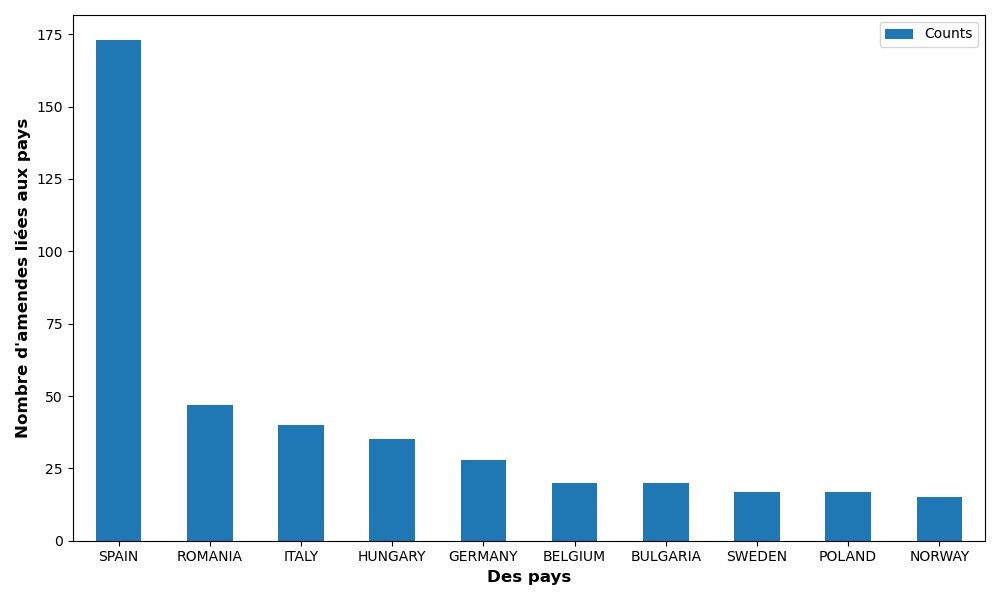
\includegraphics[width=0.7\linewidth]{graphs/top10_countries}
      \caption{Top 10 des pays de l'UE avec le plus grand nombre d'amendes}
\end{figure}
\begin{figure}
	[H]\centering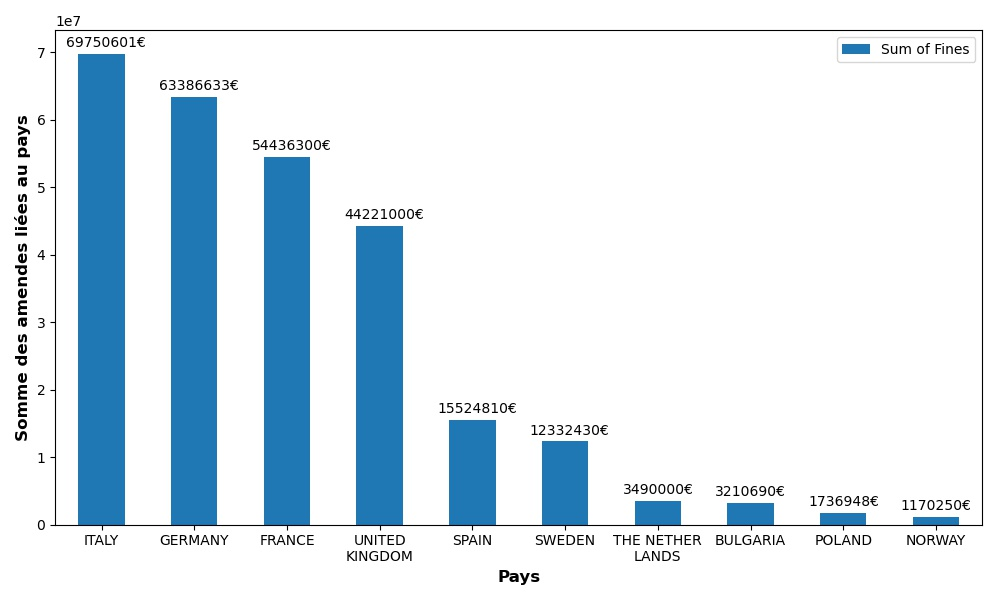
\includegraphics[width=0.7\linewidth]{graphs/top10_countries_fines}
	\caption{Top 10 des pays de l'UE avec la somme d'amendes la plus élevée}
 \end{figure}


\newpage

	\begin{multicols}{2}
	\begin{figure}
		[H]\centering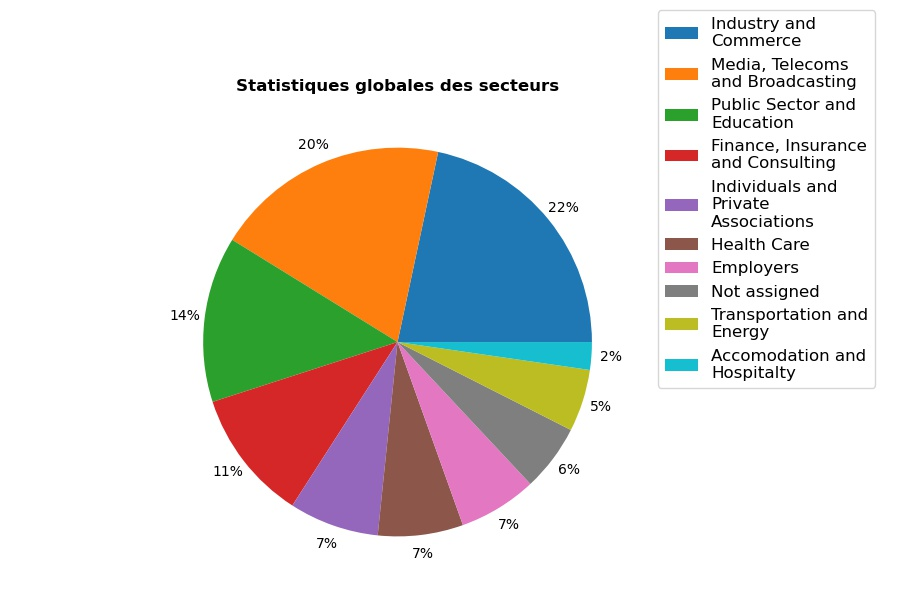
\includegraphics[width=1.0\linewidth]{graphs/sector_data}
		\caption{Top 10 des secteurs avec le plus grand nombre d'amendes}
	\end{figure}
	\begin{figure}
		[H]\centering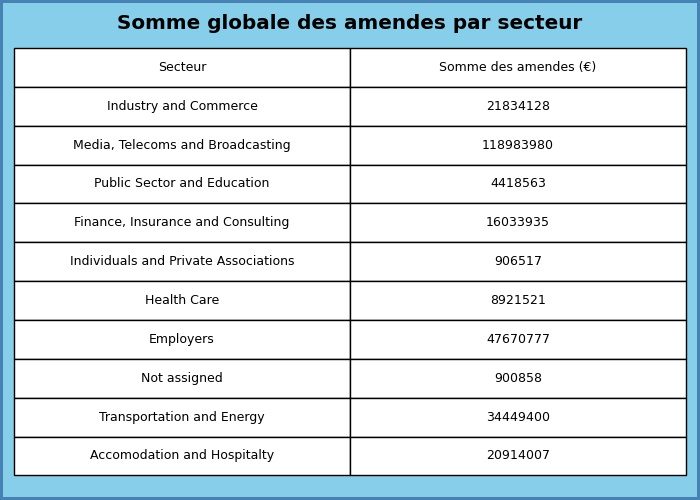
\includegraphics[width=1\linewidth]{graphs/sector_data_fines}
		\caption{Top 10 des entreprises avec le plus grand nombre d'amendes}
	 \end{figure}
	
	\end{multicols}
	
	
	
	\begin{figure}
		[H]\centering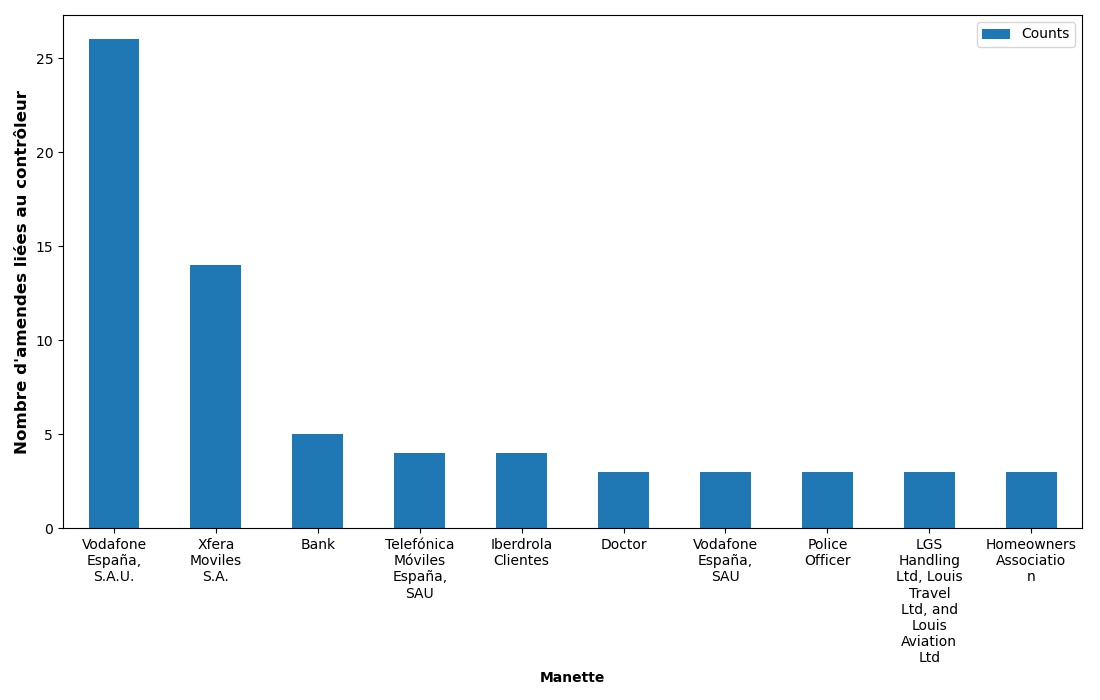
\includegraphics[width=0.6\linewidth]{graphs/top10_controller}
		\caption{Top 10 des entreprises avec le plus grand nombre d'amendes}
	\end{figure}
	
	\begin{figure}
		[H]\centering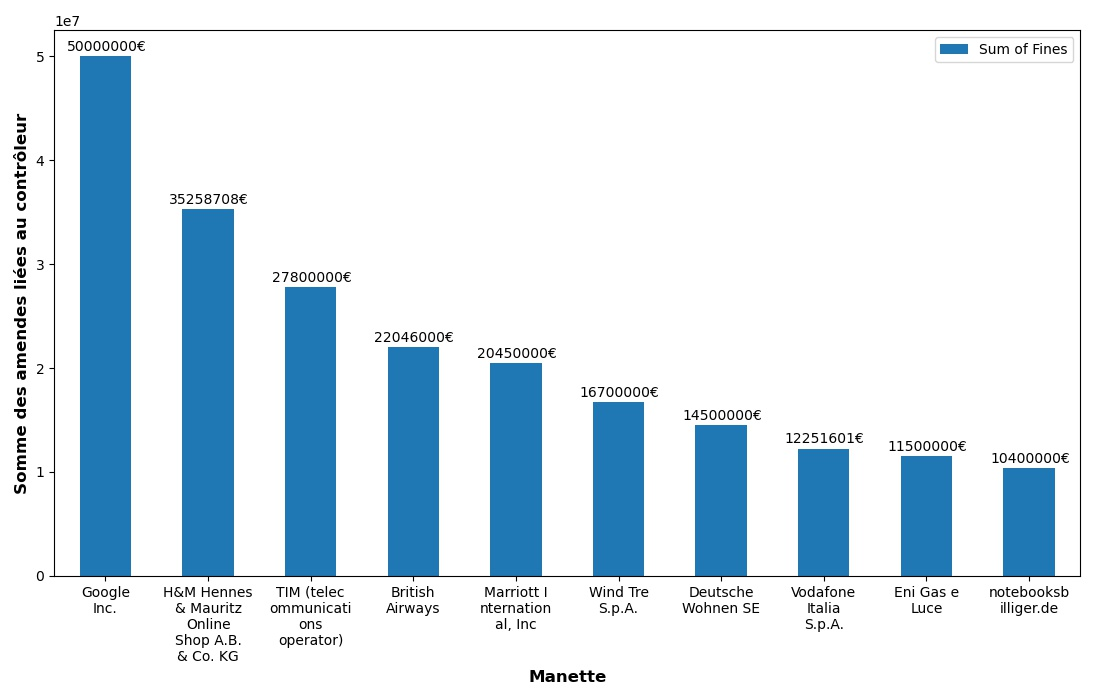
\includegraphics[width=0.6\linewidth]{graphs/top10_controller_fines}
		\caption{Top 10 des entreprises avec le montant le plus élevé d'amendes}
	 \end{figure}



\newpage


	\begin{multicols}{2}
	\begin{figure}
		[H]\centering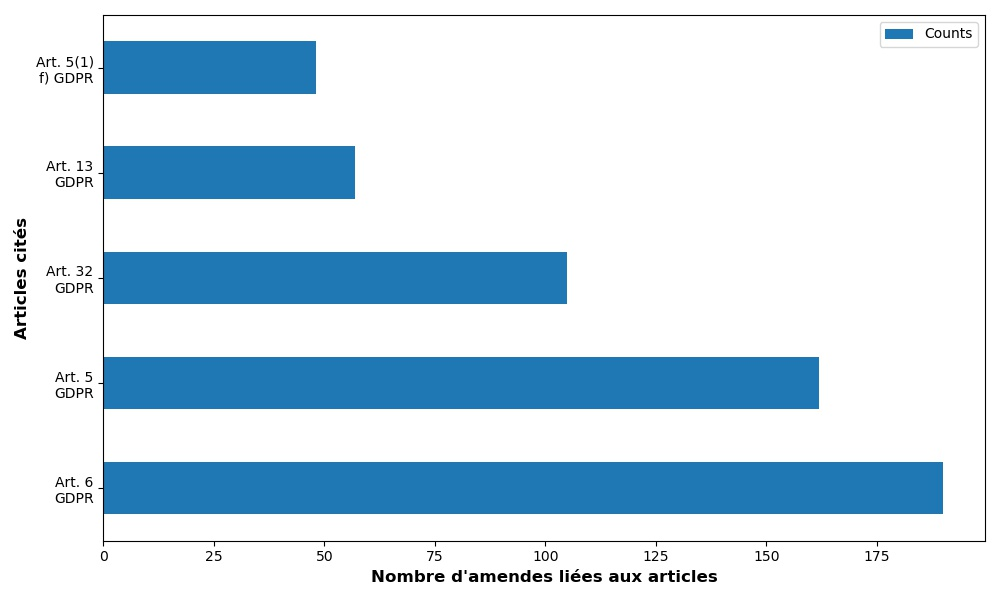
\includegraphics[width=1\linewidth]{graphs/top10_quoted} 
		\caption{Top 5 des articles cités du RGPD avec le plus grand nombre d'amendes}
	\end{figure}
	\begin{figure}
		[H]\centering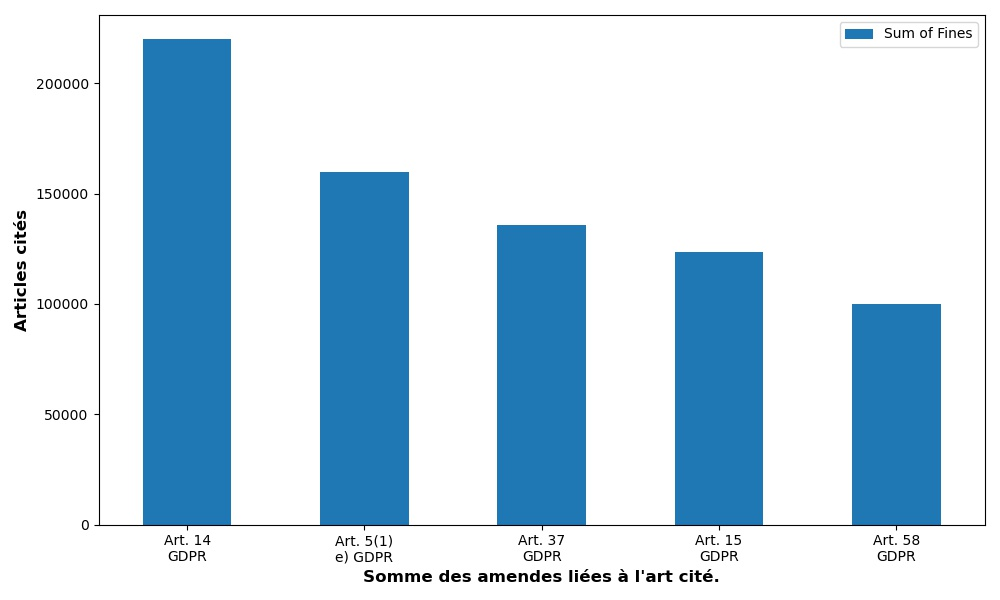
\includegraphics[width=1\linewidth]{graphs/top10_quoted_fines} 
		\caption{Top 5 des articles  du RGPD avec le montant le plus élevé d'amendes}
	\end{figure}
	\end{multicols}
	
	
	\NewsItem{\raggedright{\LARGE Analyse sur l'application du RGPD au fil des ans}}
	\begin{figure}
		[H]\centering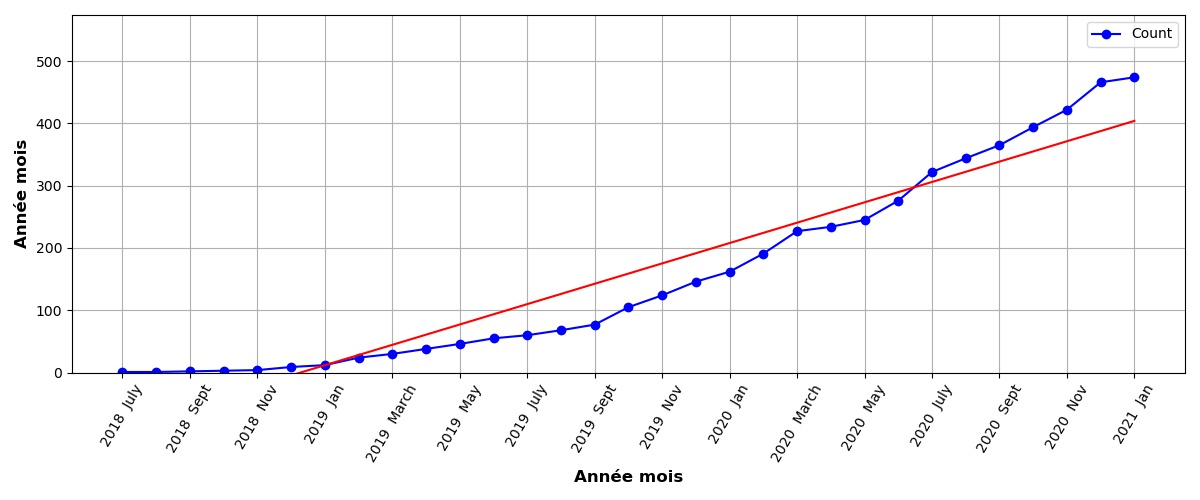
\includegraphics[width=0.8\linewidth]{graphs/acc_nb_cases_graph}
		\caption{Le nombre d'amendes (cumulatif) }
	\end{figure}
	
	\begin{multicols}{2}
	\begin{figure}
		[H]\centering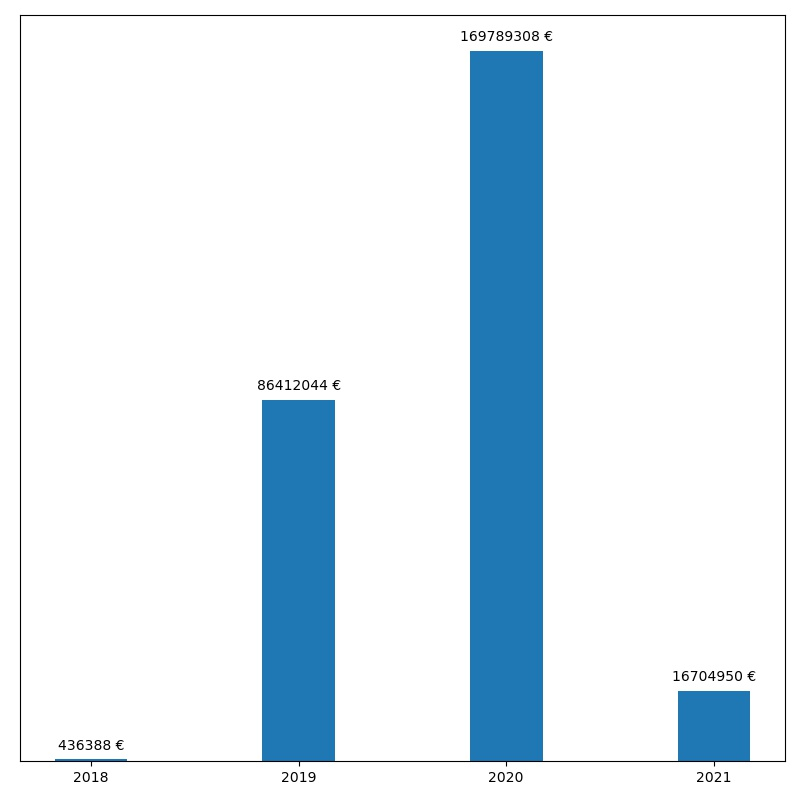
\includegraphics[width=1.0\linewidth]{graphs/SumOfFinesperYear}
		\caption{La somme d'amende par an }
	 \end{figure}
\justify
	L'application du RGPD s'est accélérée depuis les premières années, tant sur le nombre de cas d'exécution que sur la somme des amendes. La sensibilisation du public et la couverture médiatique de la vie privée et de la protection des données se sont également accrues au fil des ans. Cependant, le RGPD risque d'échouer. Selon une étude de Brave, cela est dû au fait que les autorités de protection des données (DPA) ne donnent pas suffisamment de ressources humaines et financières pour accomplir leurs tâches. Seuls 6 DPA nationaux disposent de plus de 10 enquêteurs techniques spécialisés. La moitié de toutes les APD nationales reçoivent de petits budgets annuels (5 millions d'euros ou moins) de leurs gouvernements.
	\end{multicols}



\newpage



%Particular Year Statistic
\NewsItem{\raggedright{\LARGE Amendes RGPD Sanctionnées en 2018}}

	\begin{multicols}{2}
	
	En 2018,  il y a eu \textbf{12} amendes.
	Le total cumulé des amendes de protection des données pour 2018 se tient maintenant à \textbf{458 688€}.
	
	\begin{figure}[H]
	\centering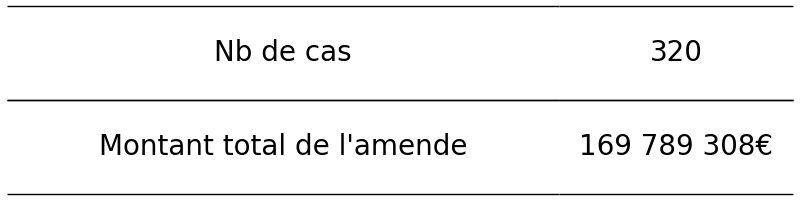
\includegraphics[width=1\linewidth]{graphs/counter_year}
	\end{figure}


	Les amendes du RGPD pour 2018 se résume pour chaque mois comme suit :

	\begin{figure}
	[H]\centering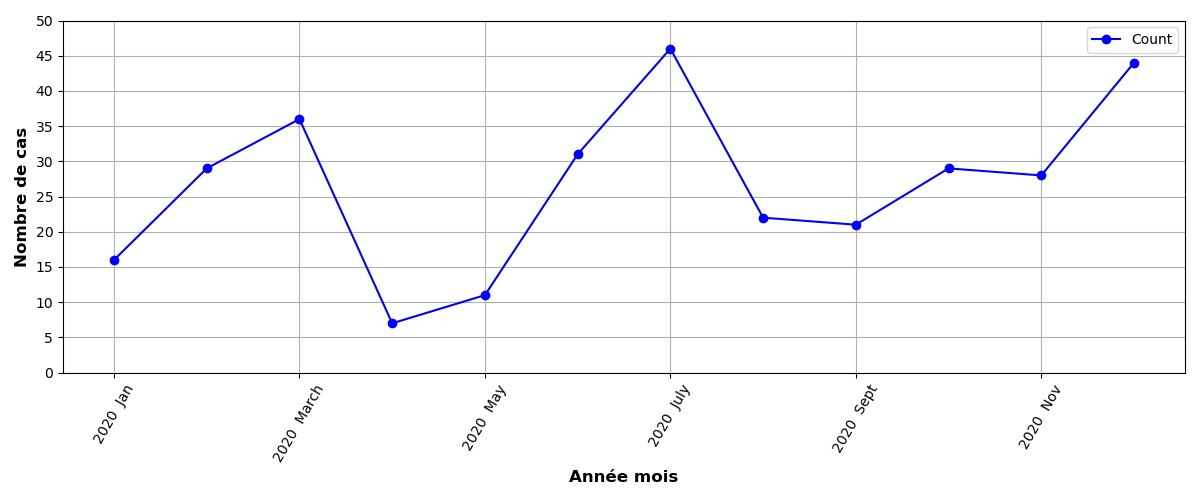
\includegraphics[width = 1.2\linewidth]{graphs/NbFinesPerMonth_year_graph}
	\caption{Petit aperçu sur des mois 2018}
	\end{figure}

	\end{multicols}


	\begin{figure}
		[H]\centering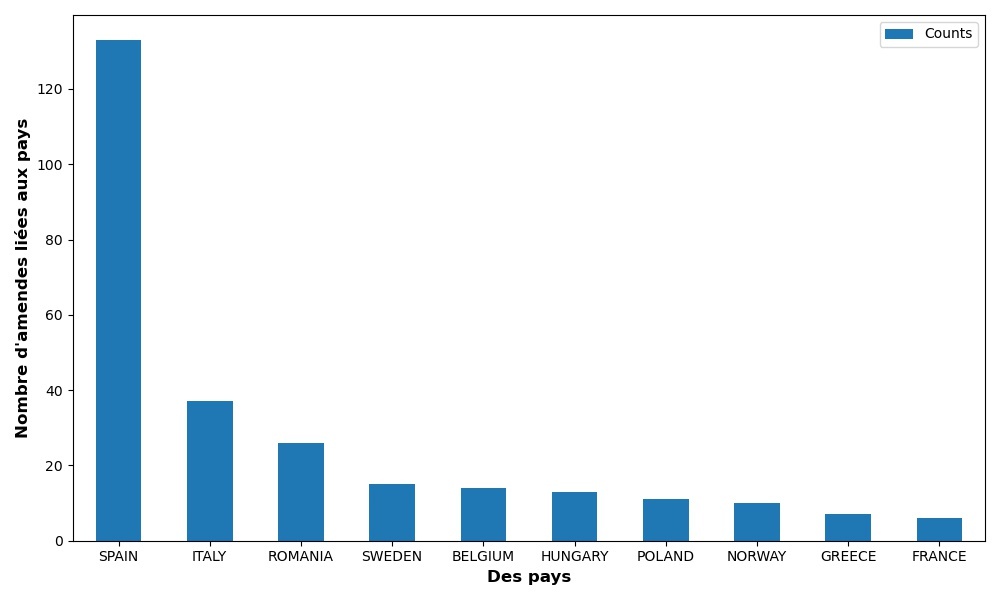
\includegraphics[scale=.5]{graphs/top10_countries_year}
		\caption{Top 10 des pays de l'UE avec le plus grand nombre d'amendes en 2018}
	\end{figure}
	\begin{figure}
		[H]\centering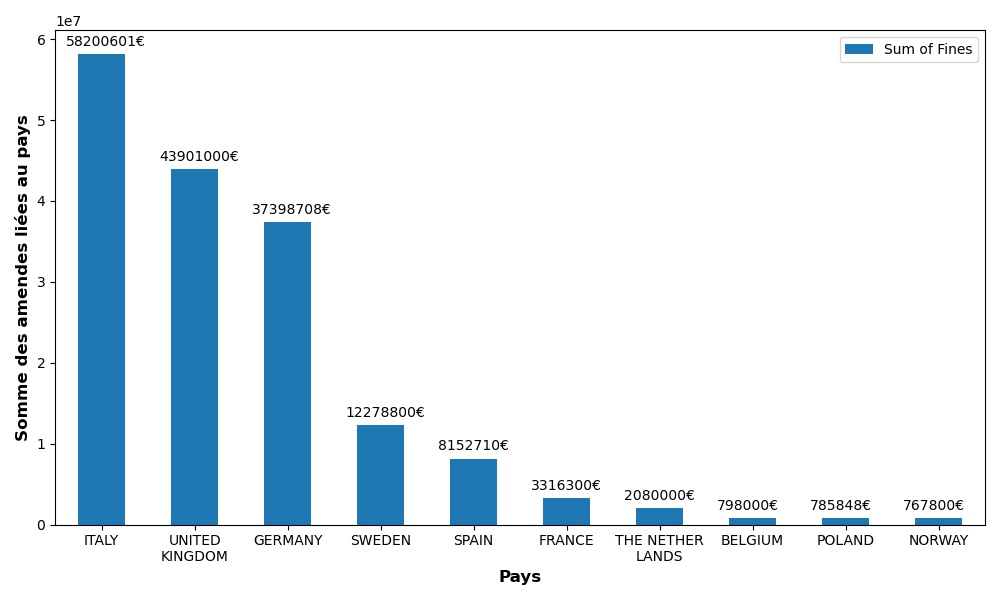
\includegraphics[scale=.5]{graphs/top10_countries_year_fines}
		\caption{Top 10 des pays de l'UE avec la somme d'amendes la plus élevée en 2018}
	\end{figure}

\newpage
\justify
	\begin{multicols}{2}
	\heading{3 amendes les plus récentes en 2018}{3 pt}
		\begin{itemize}
			\item \textbf{2018-12-20} \newline
			2,200€ d'amende en L'AUTRICHE pour Personne privée.
			\newline
			L'amende a été infligée à un particulier qui utilisait la vidéosurveillance à son domicile.
			\newline
			\href{https://www.ris.bka.gv.at/Dokumente/Dsk/DSBT_20181220_DSB_D550_037_0003_DSB_2018_00/DSBT_20181220_DSB_D550_037_0003_DSB_2018_00.pdf}{Plus d'informations}
			\vspace{1cm}
	
			\item \textbf{2018-12-18} \newline
			3,200€ d'amende en HONGRIE pour Inconnue.
			\newline
			L'amende a été infligée pour (i) ne pas avoir fourni à une personne concernée des enregistrements de vidéosurveillance, (ii) ne pas conserver les enregistrements pour une utilisation ultérieure par la personne concernée, et (iii) ne pas avoir informé la personne concernée de son droit de déposer une plainte auprès du contrôle.
			\newline
			\href{https://www.naih.hu/files/NAIH-2018-5559-H-hatarozat.pdf}{Plus d'informations}
			\vspace{1cm}
	
			\item \textbf{2018-12-17} \newline 5,000€ d'amende en ALLEMAGNE pour Image de Kolibri
			\newline
			Remarque: selon nos informations, cette amende a été retirée entre-temps.
			\newline
			\href{https://www.heise.de/newsticker/meldung/DSGVO-5000-Euro-Bussgeld-fuer-fehlenden-Auftragsverarbeitungsvertrag-4282737.html}{Plus d'informations}
		\end{itemize}
	\end{multicols}

\newpage
\justify
	\begin{multicols}{2}
		\heading{Amendes notables in 2018}{3 pt}
	\begin{itemize}
		\item \textbf{La plus grosse amende} en 2018 - \textbf{400000 €} a été condamné par LE PORTUGAL à Hôpital public.
		\newline
		\textbf{Résumé} : L’enquête a révélé que le personnel de l’hôpital, les psychologues, les diététistes et d’autres professionnels avaient accès aux données des patients au moyen de faux profils.
		\newline
		\href{https://www.cnpd.pt/bin/decisoes/Delib/20_984_2018.pdf}{Plus d'informations}
		\vspace{1cm}
	
		\item \textbf{La plus petite amende} en 2018 - \textbf{300 €} -  a été condamné par  à Propriétaire de voiture privée.
		\newline
		\textbf{Résumé} : Une Dashcam a été utilisée illégalement.
		\newline
		\href{https://www.ris.bka.gv.at/Dokumente/Dsk/DSBT_20180927_DSB_D550_084_0002_DSB_2018_00/DSBT_20180927_DSB_D550_084_0002_DSB_2018_00.pdf}{Plus d'informations}
	\end{itemize}
	\end{multicols}


\newpage

	
	\begin{multicols}{2}
	\begin{figure}
		[H]\centering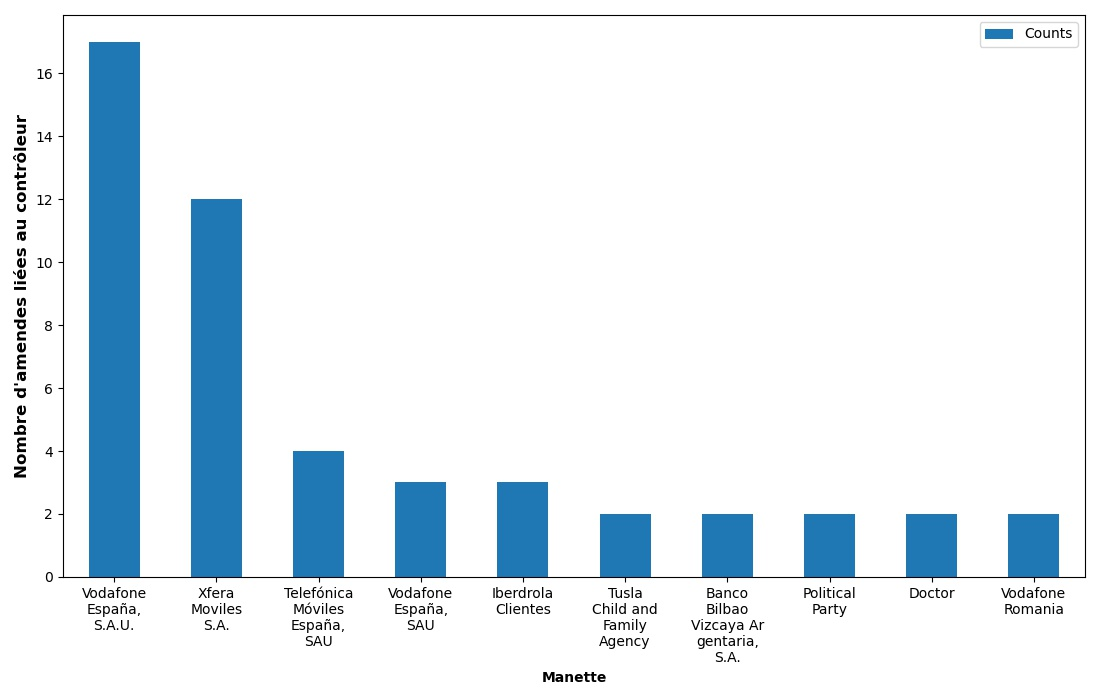
\includegraphics[width=1.0\linewidth]{graphs/top10_controller_year}
		\caption{Top 10 des entreprises avec le plus grand nombre d'amendes en2018}
	\end{figure}
	\begin{figure}
		[H]\centering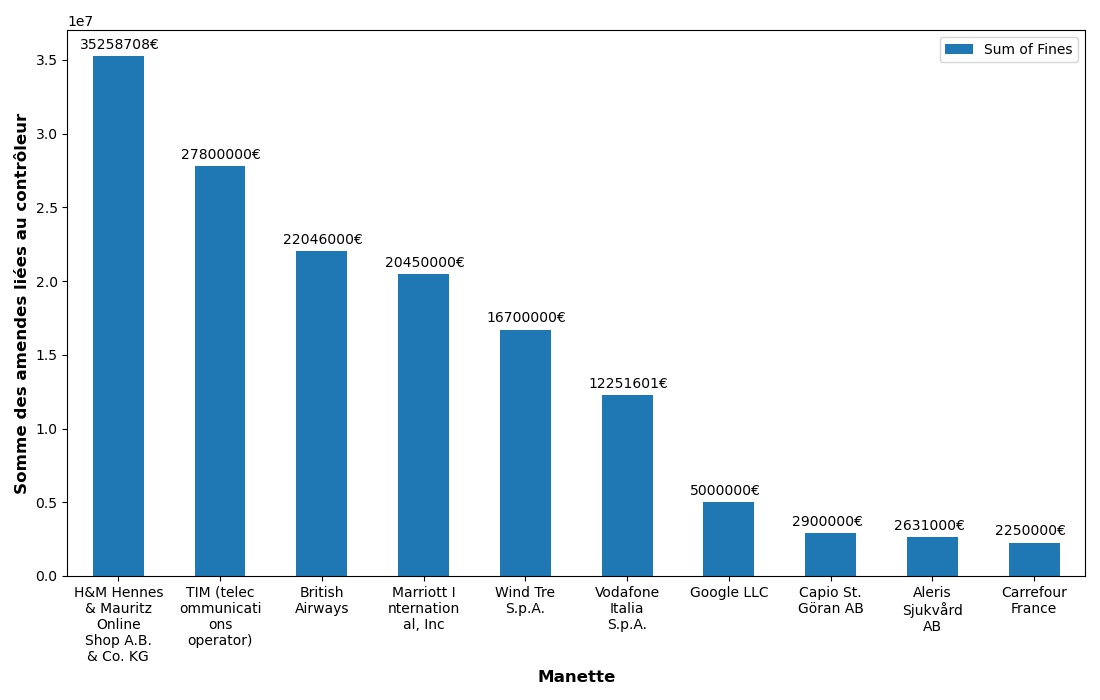
\includegraphics[width=1\linewidth]{graphs/top10_controller_year_fines}
		\caption{Top 10 des entreprises avec le montant le plus élevé d'amendes en 2018}
	 \end{figure}
	
	\end{multicols}


		
	\begin{multicols}{2}
	\begin{figure}
		[H]\centering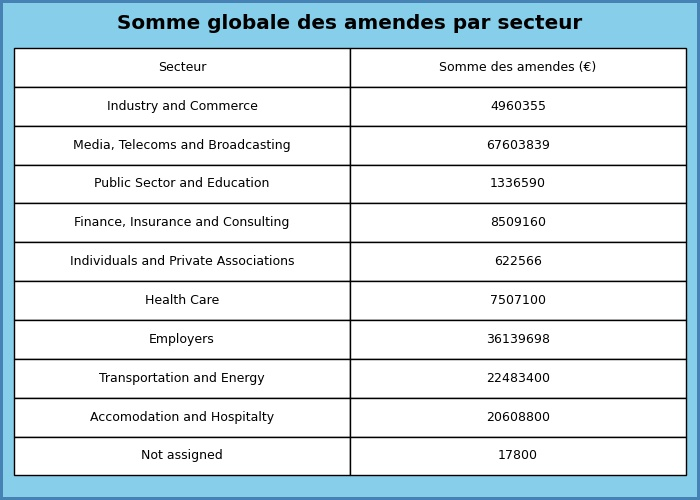
\includegraphics[width=1.0\linewidth]{graphs/sector_data_year_fines}
		\caption{Top 10 des secteurs avec le montant le plus élevé d'amendes2018}
	\end{figure}
	\begin{figure}
		[H]\centering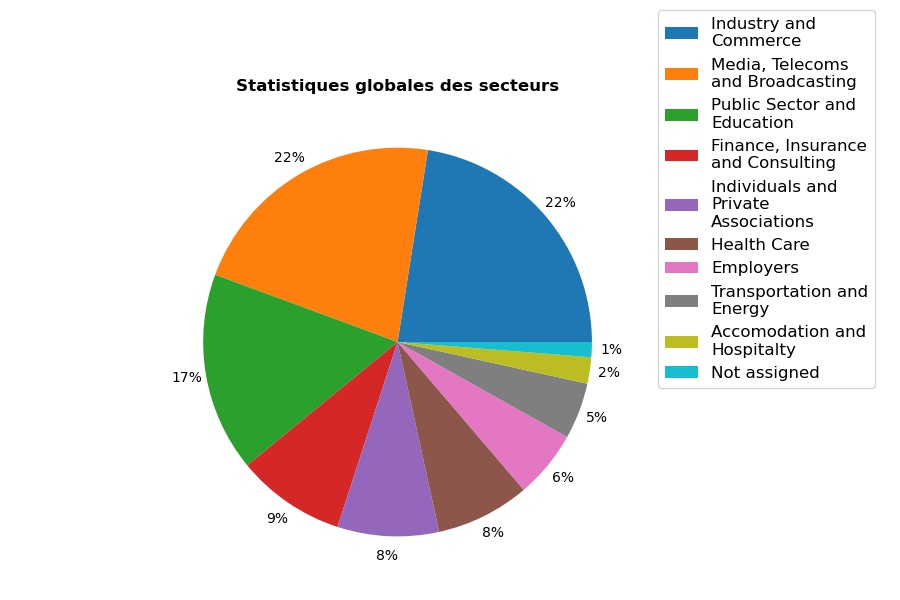
\includegraphics[width=1\linewidth]{graphs/sector_data_year}
		\caption{Top 10 des secteurs avec le montant le plus élevé d'amendes2018}
	 \end{figure}
	
	\end{multicols}

	\begin{multicols}{2}
	\begin{figure}
		[H]\centering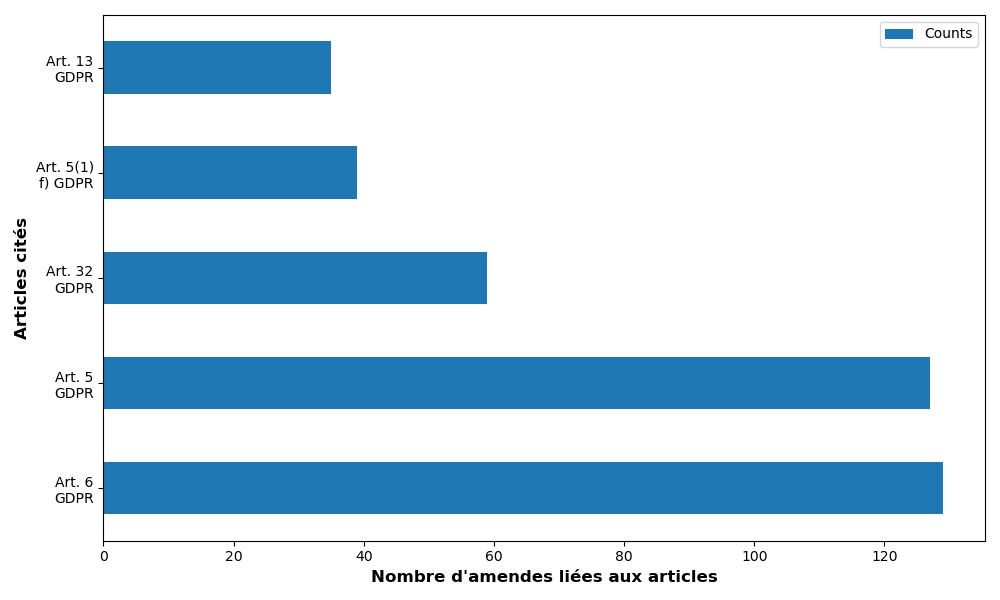
\includegraphics[width=1.0\linewidth]{graphs/top10_quoted_year}
		\caption{Top 5 des articles cités du RGPD avec le plus grand nombre d'amendes en 2018}
	\end{figure}
	\begin{figure}
		[H]\centering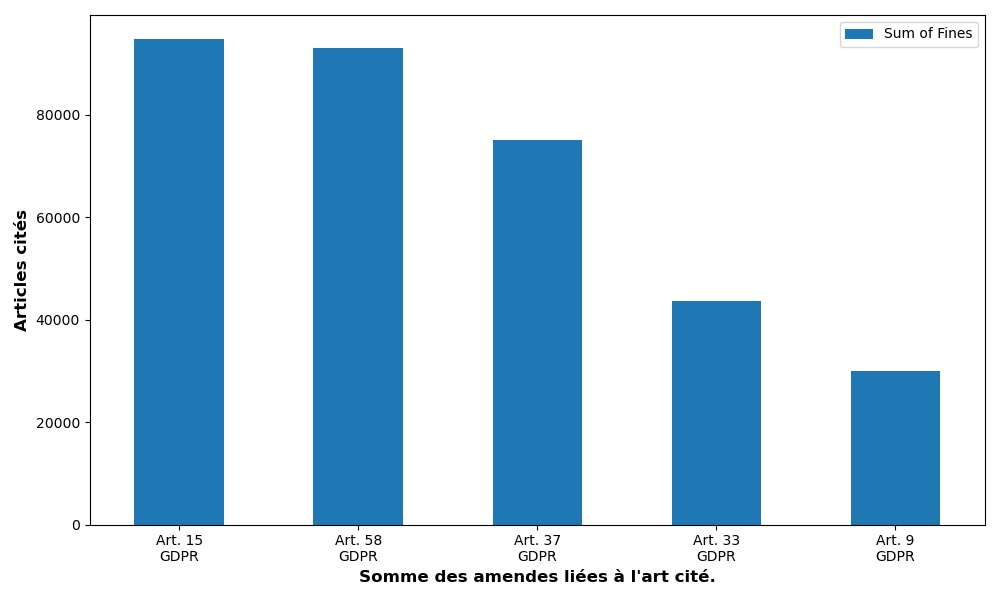
\includegraphics[width=1\linewidth]{graphs/top10_quoted_year_fines}
		\caption{Top 5 des articles  du RGPD avec le montant le plus élevé d'amendes en 2018}
	 \end{figure}
	
	\end{multicols}









\vspace*{\fill}
\textbf{Références:}\\
\href{https://www.enforcementtracker.com}{https://www.enforcementtracker.com}\\
\href{https://brave.com/wp-content/uploads/2020/04/Brave-2020-DPA-Report.pdf}{https://brave.com/wp-content/uploads/2020/04/Brave-2020-DPA-Report.pdf}\\
\href{https://arxiv.org/pdf/2011.00946.pdf}{https://arxiv.org/pdf/2011.00946.pdf}


\end{document}